\section{Reynolds effects}
We are now interested to catch the effects of the Reynolds on our statistics through the comparison of our two simulations.\\~\par
The first macroscopical effect that we face is a shift, towards higher values, of the mean velocity profile. The shadowed area of the graph~\ref{mean:comparison} depict such situation. According to this figure, we can see a narrowing of the region subjected to high viscous stress, as the Reynolds number becomes larger.\par
Under the mean velocity profile graph we reported the same quantity, but presented in semi-logaritmic scale, using both inner and outer scaling.
The first plot of figure~\ref{loglaw:comparison} correlates the results of the simulations and the theoretical behavior expectations.
In particular we can see that, despite the Reynolds number, all the simulations present the linear $\bar{u}=y^{+}$ behavior expected in the viscous sublayer, and the logarithmic profile in the homonym region, with $k=0.41$ and $B=5.2$.\\~\par

\begin{figure}
\begin{center}
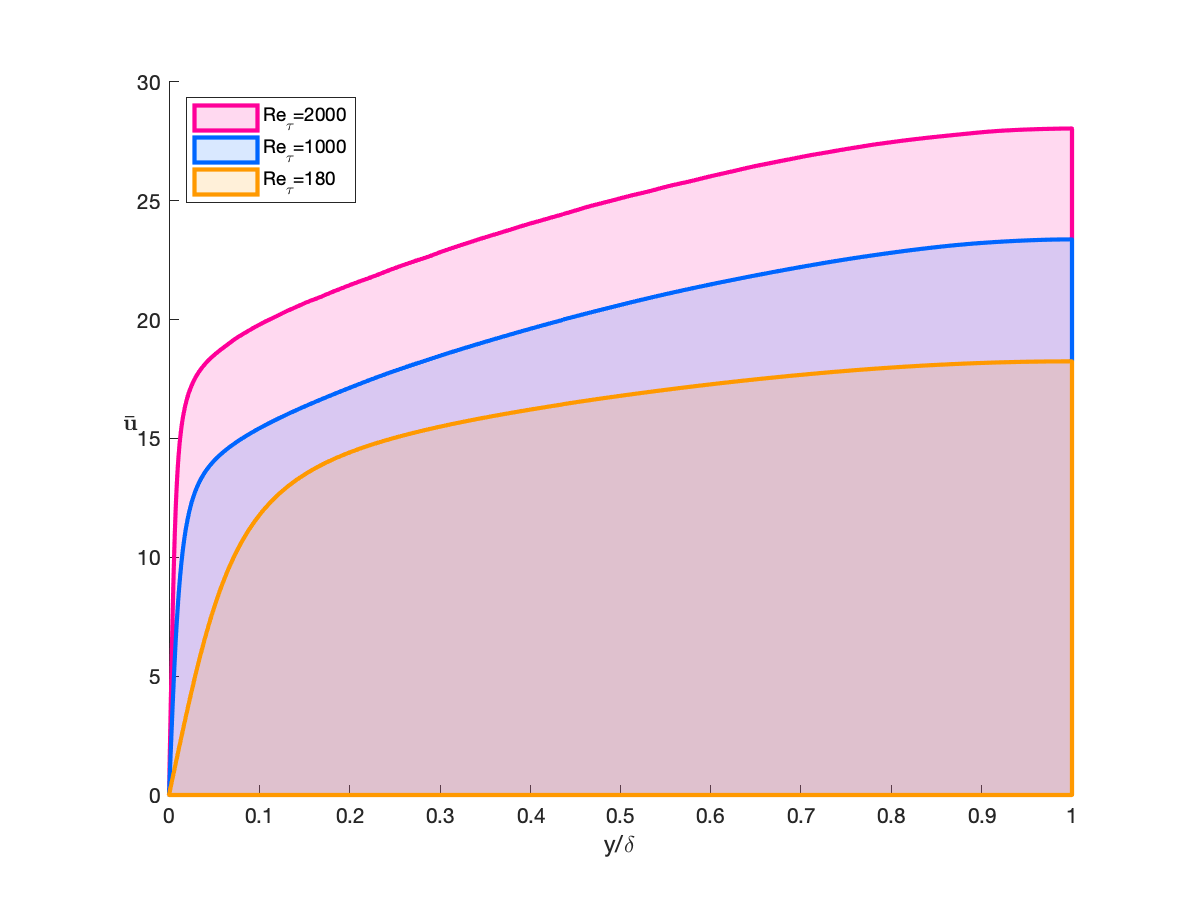
\includegraphics[scale=0.55]{grafici/u_mean_comparison.eps}
\caption{Mean velocity profile at $Re_{\tau}$ variation}
\label{mean:comparison}
\end{center}
\end{figure}
\begin{figure}
\begin{center}
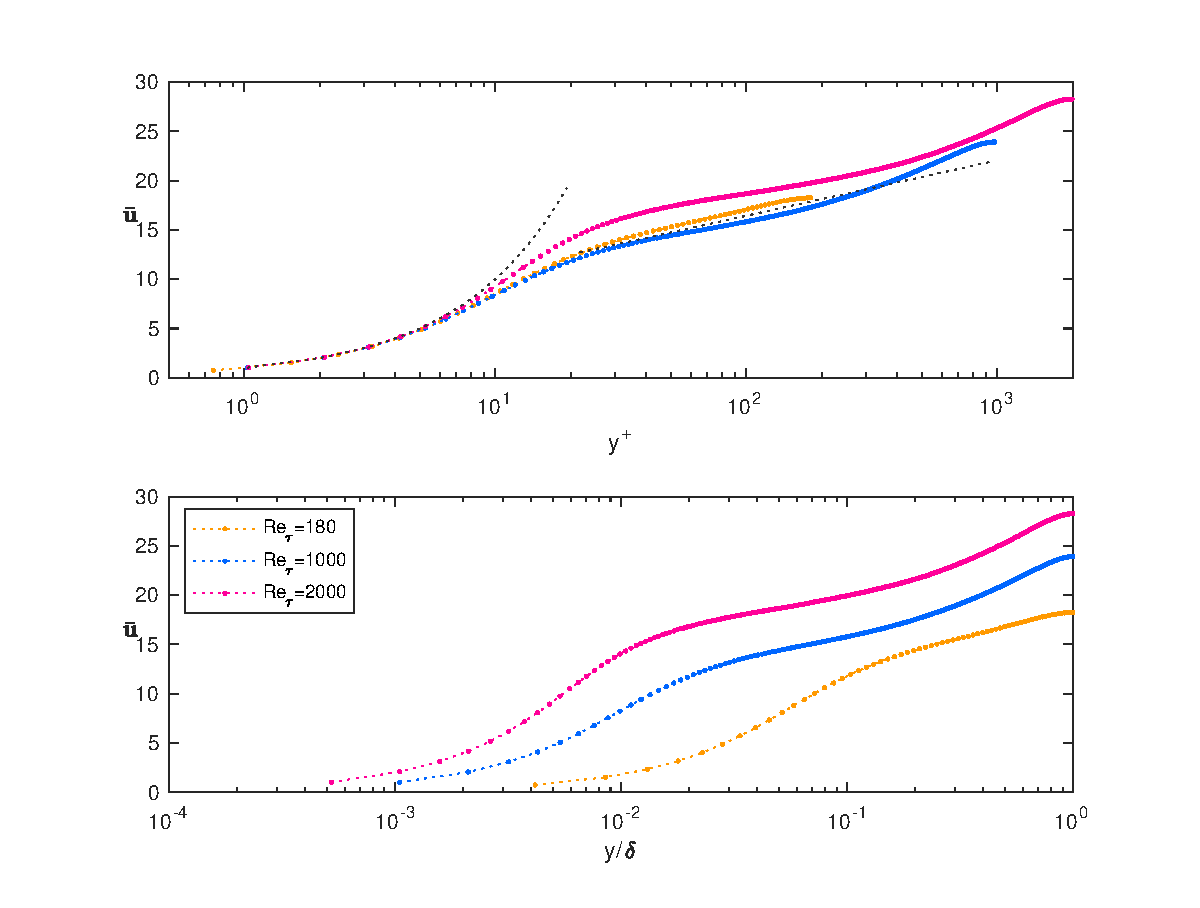
\includegraphics[scale=0.55]{grafici/loglaw_comparison.eps}
\caption{The law of the wall, in inner and outer scaling, at $Re_{\tau}$ variation}
\label{loglaw:comparison}
\end{center}
\end{figure}

Figure~\ref{shear:comparison} shows how the shear stress components modify as the Reynolds number increase. \par
Focusing on the normalized Reynolds stress curve we can clearly see that, as the $Re_{\tau}$ increase, the region subjected to this kind of stress becomes larger, with the peak moving towards the wall. Such kind of stress is associated with the fluid turbulent motions, therefore it was expectable a raise of this components as we move towards a more turbulent flow. \par

\begin{figure}
\begin{center}
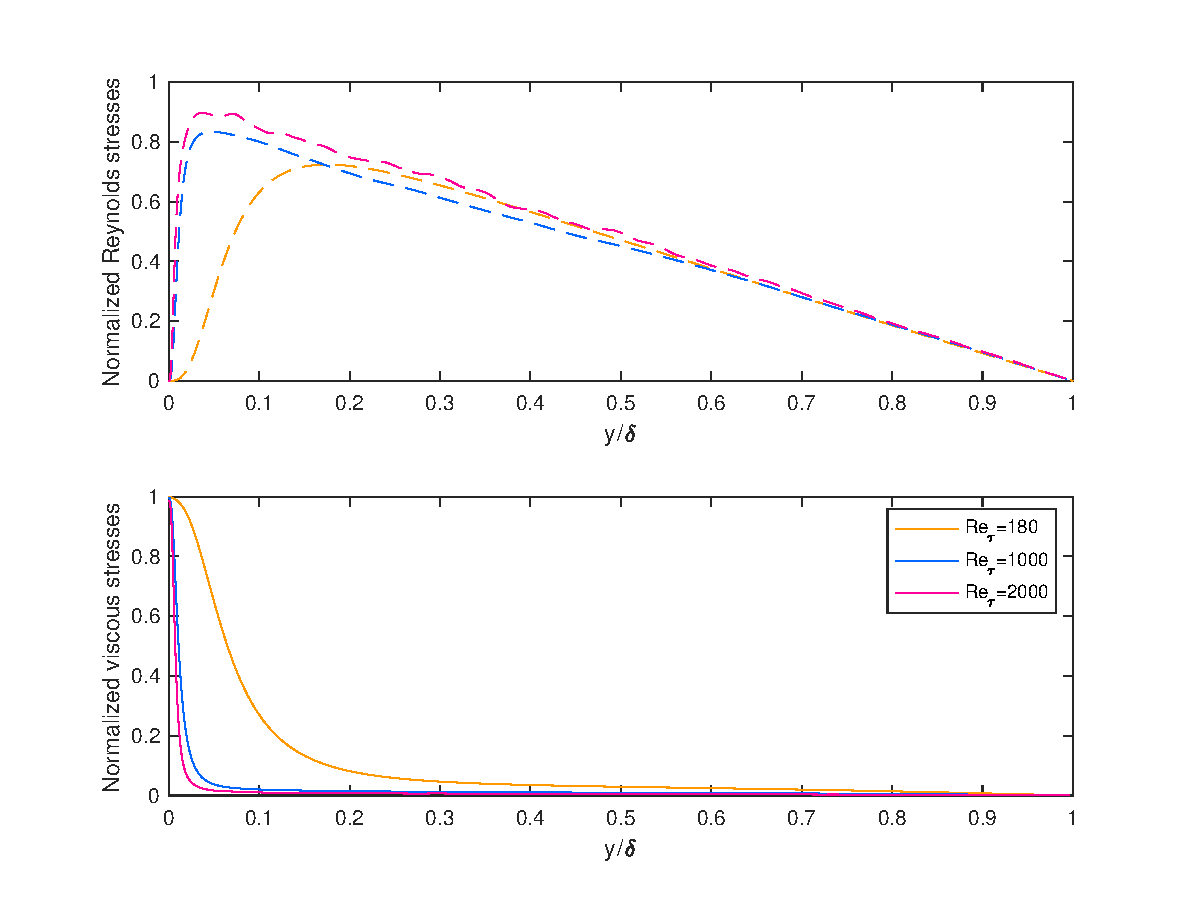
\includegraphics[scale=0.55]{grafici/shear_comparison.eps}
\caption{Normalized shear profiles at $Re_{\tau}$ variation}
\label{shear:comparison}
\end{center}
\end{figure}

\begin{figure}
\begin{center}
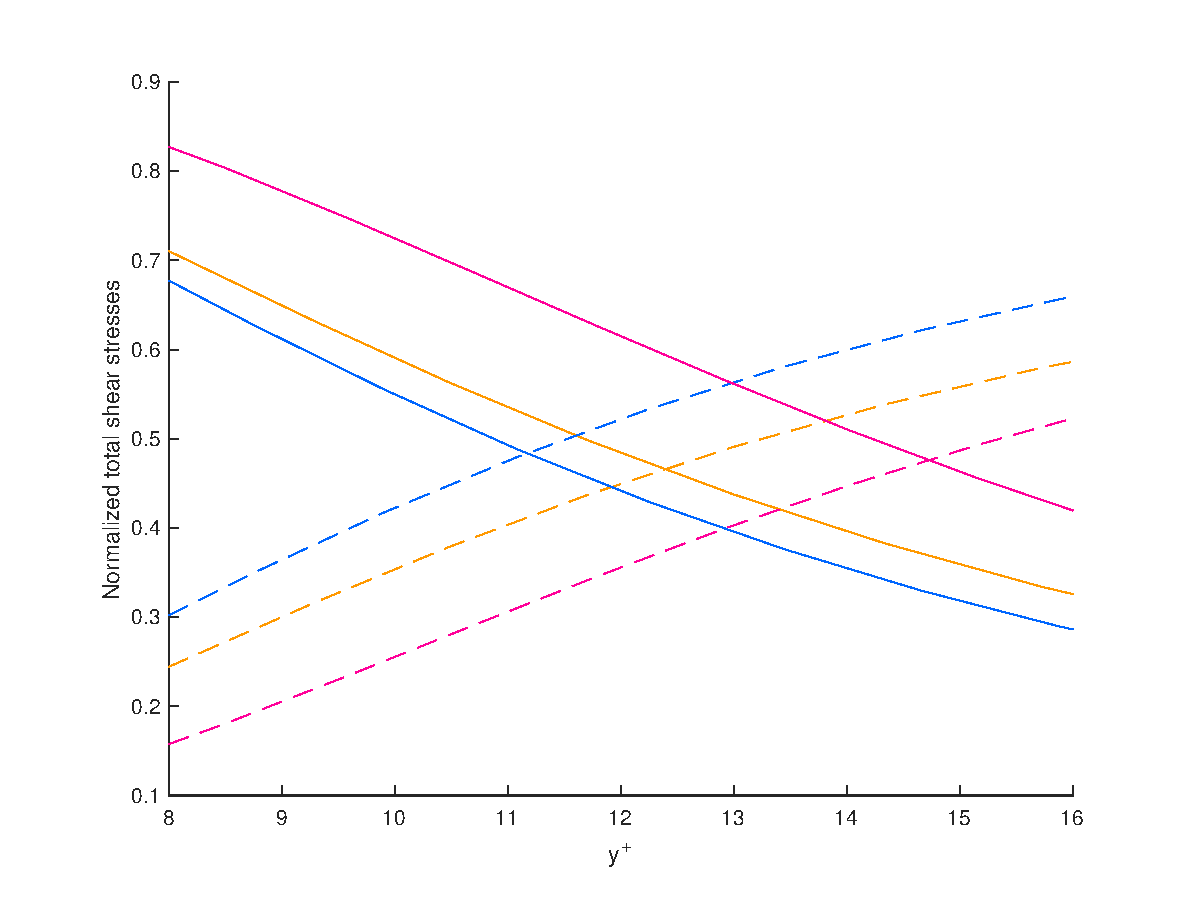
\includegraphics[scale=0.55]{grafici/y12.eps}
\caption{Particular of the shear stress, at $Re_{\tau}$ variation}
\label{y12}
\end{center}
\end{figure}

On the other hand the contribute of the viscous stress, associate to $\partial{\bar{u}}/\partial{t}$, is maximum at the wall and tends to become negligible as we move towards the centerline. \par
As testified by figure~\ref{loglaw:comparison}, the higher is the Reynolds and the wider is the area subjected to logarithmic profile, hence smaller is the area subjected to strong variation of the mean velocity profile with the wall-normal coordinate. This fact reflects on our viscous shear component reducing its range of effectiveness to few units, close to the wall, as the $Re$ grows.\par
Although, in terms of outer scaling, the stress components are subjected to strong variations, in inner scaling we can see, in figure~\ref{y12}, that the point at which the two components cross themself remains quite constant, with $y^{+}\approx$ 12 wall-units. \\~\par


\begin{figure}
\begin{center}
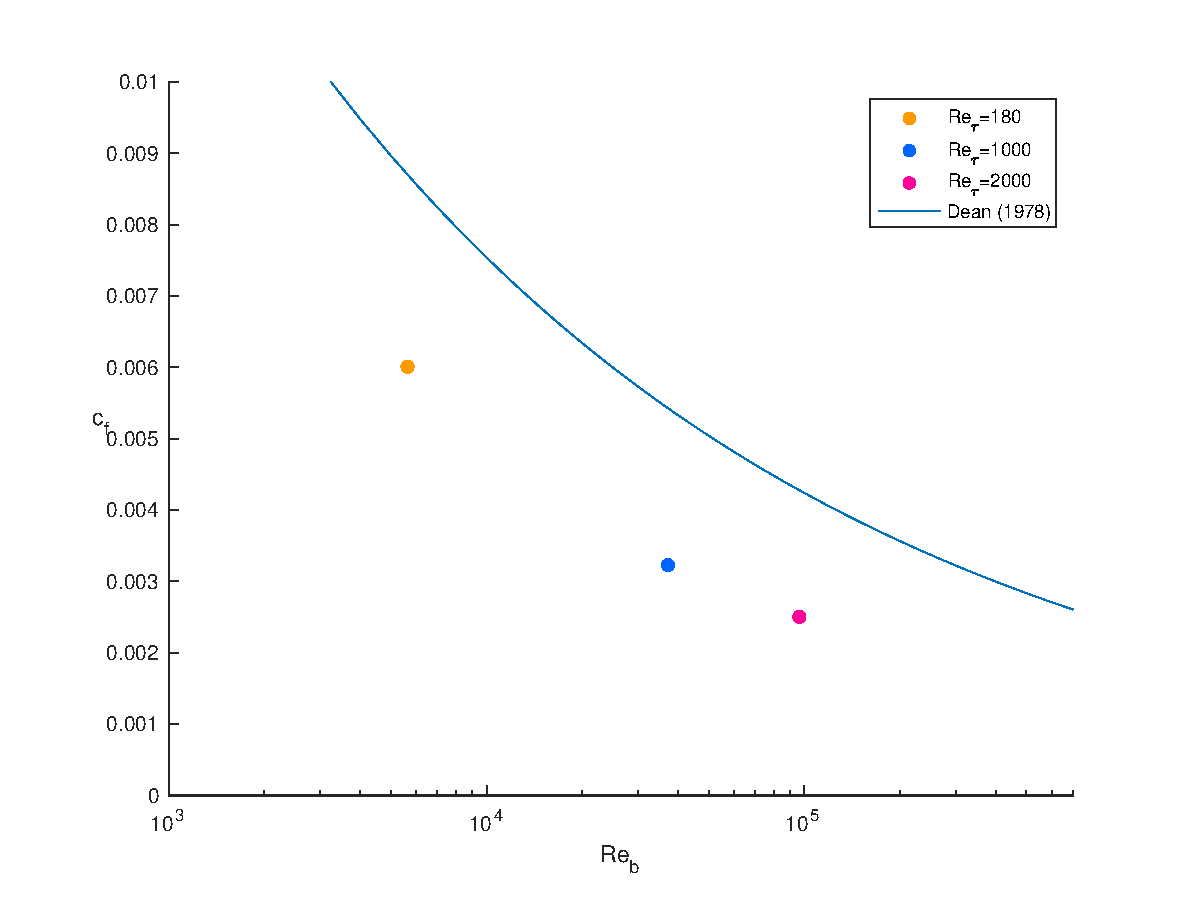
\includegraphics[scale=0.55]{grafici/cf.eps}
\caption{Dependance of the $c_{f}$ from $Re_{b}$}
\label{cf}
\end{center}
\end{figure}


One of the most important flow property for wall bounded flows is the friction coefficient.
The $c_{f}$ has been studied in detail by many famous authors of the past: Nikuradse, Prandtl, Blasius just to cite some of them. \par
In our simulations we computed the skin friction coefficient through the definition provided by~\cite[279]{pope}, which is based on centerline velocity $(U_{0})$ and the $Re_{b}$ of the channel.
The quantities have been defined as
\begin{equation*}
c_{f}= 2(\frac{u_{\tau}}{U_{0}})^{2}	\quad~\quad~\quad~\quad	Re_{b}= \frac{2 U_{b} \delta}{\nu},
\end{equation*}
and the results have been reported on figure~\ref{cf}. \par
Our $c_{f}$ shows good fitting with the results of the experimental campaign of Dean reported in~\cite{Dean}.\\~\par

\begin{figure}
\begin{center}
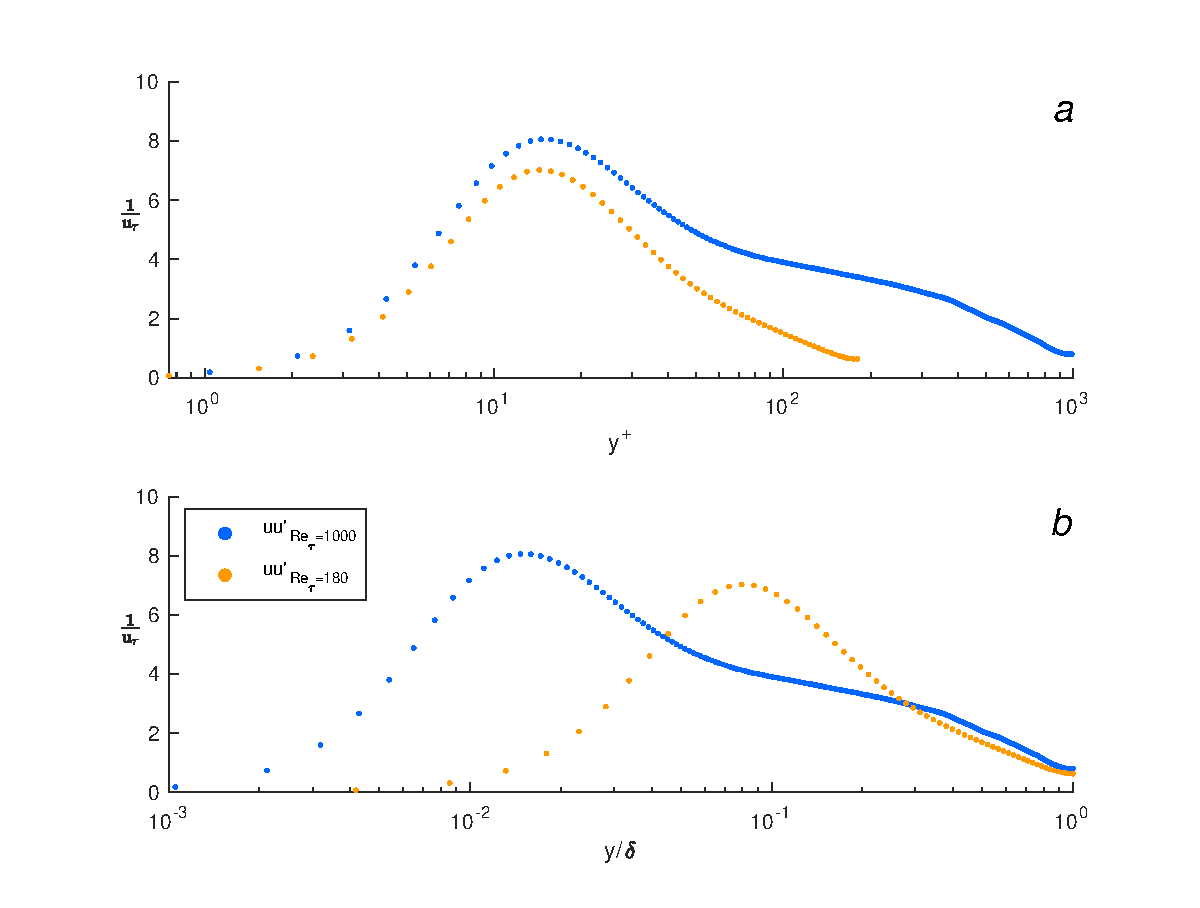
\includegraphics[scale=0.55]{grafici/uu_comparison.eps}
\caption{Streamwise fluctuations as function of the distance from the wall, plotted at $Re_{\tau}$ variation}
\label{uu:comparison}
\end{center}
\end{figure}
\begin{figure}
\begin{center}
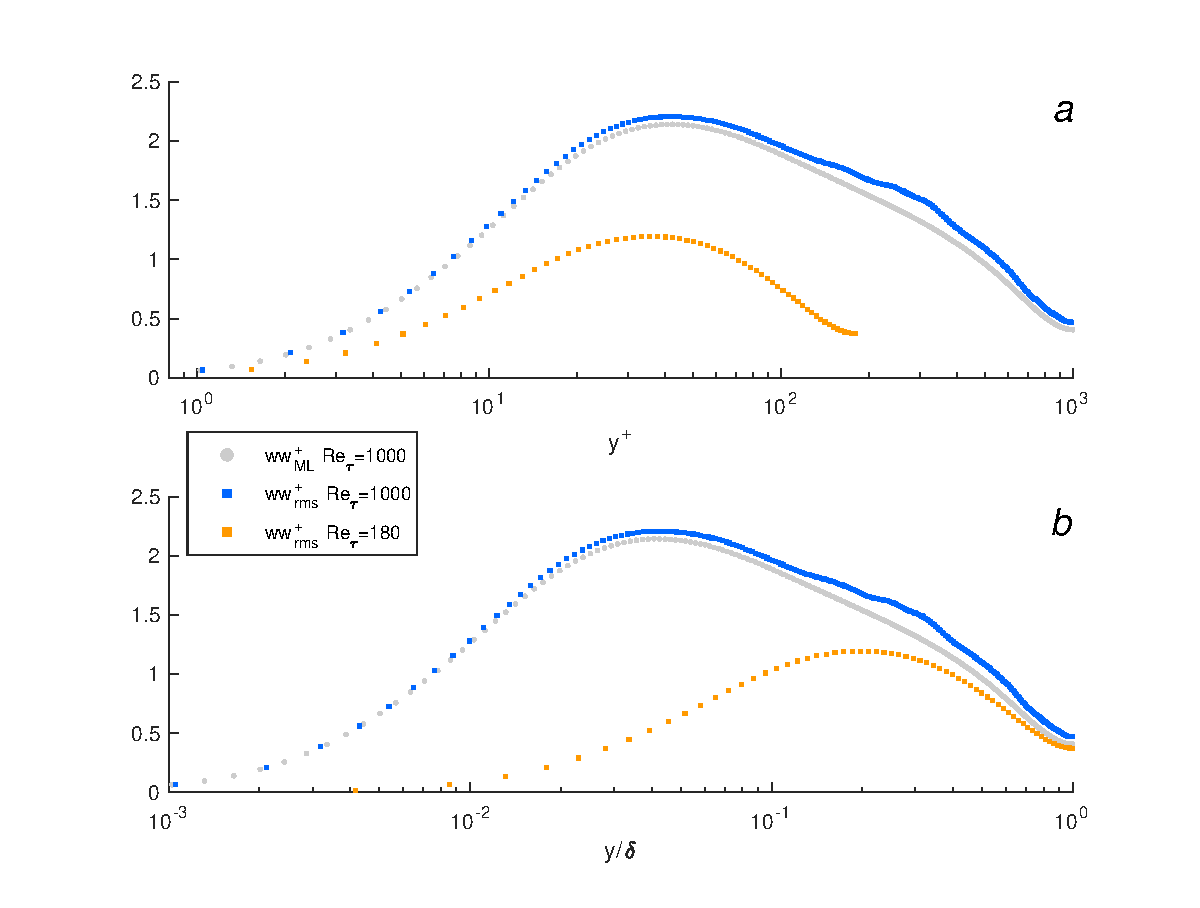
\includegraphics[scale=0.55]{grafici/ww_comparison.eps}
\caption{Spanwise fluctuations as function of the distance from the wall, plotted at $Re_{\tau}$ variation}
\label{ww:comparison}
\end{center}
\end{figure}

Let introduce now the comparison among the \emph{rms} terms. \par
Figure~\ref{ww:comparison} shows the fluctuations of the spanwise term. As we can catch from the first plot, the raise of the Reynolds number, aside of the shift towards higher values, have a crucial effect on the trailing profile of the curve. Indeed we can appreciate the born of a logarithmic region for $w'^{2}$ term. In order to identify such region, we have used an estimator function defined as $y\partial_{y}\langle w'^{2} \rangle$, suggested in~\cite{Lee}. This function has the peculiarity to exhibit a flat profile whereas a logarithmic behavior is present.\par

In figure~\ref{d2:rms}\emph{d} we can see that the blue profile, which indicates the $Re_{\tau}=1000$ simulation exhibit a flat path around $y^{+}\approx100$, in agreement to what is shown in figure~\ref{ww:comparison} and predicted in~\cite{Lee}.
The analysis for $Re_{\tau}=180$ simulation does not highlight similar behaviors.\\~\par

\begin{figure}
\begin{center}
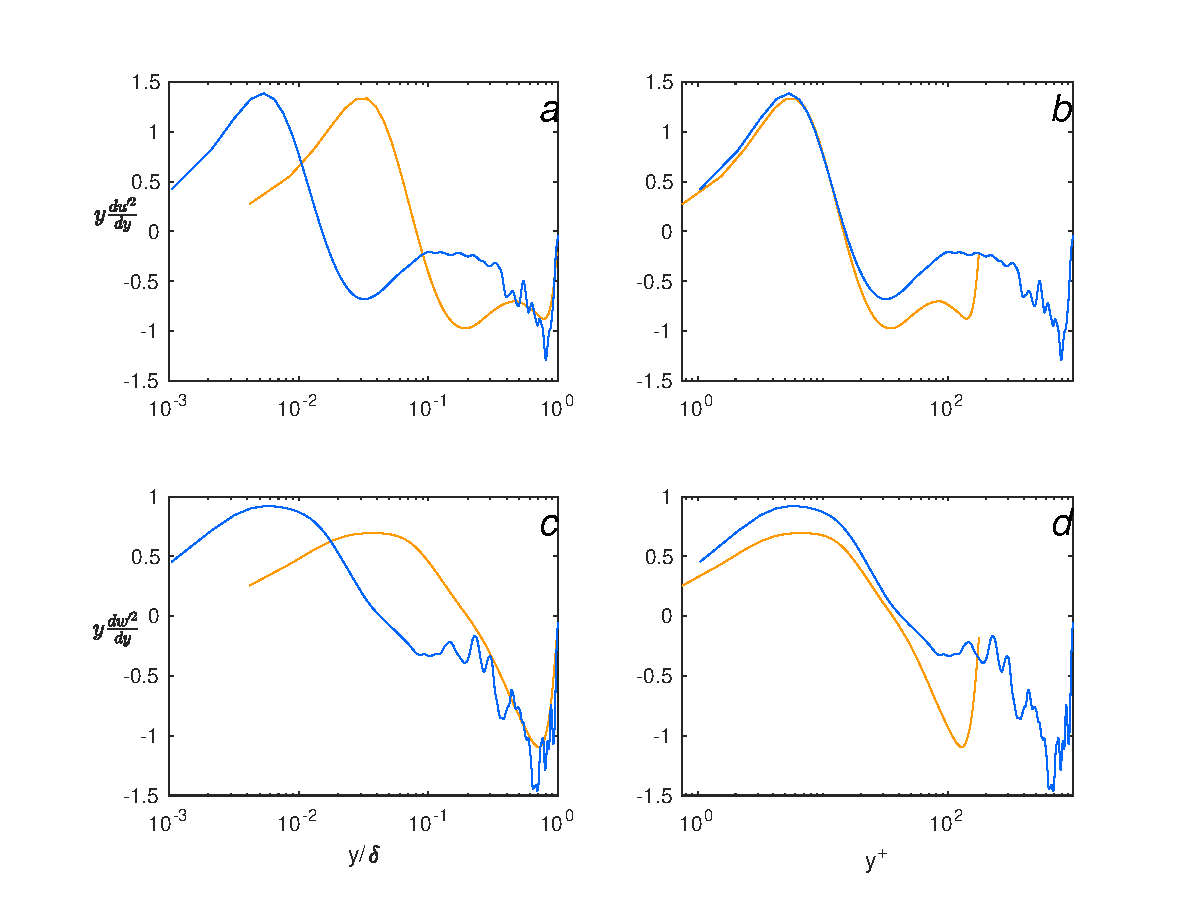
\includegraphics[scale=0.55]{grafici/d2rms.eps}
\caption{Spanwise and streamwise logarithmic region predictor. For legend refer to \ref{uu:comparison}}
\label{d2:rms}
\end{center}
\end{figure}

For what concern the streamwise fluctuations, reported in figure~\ref{d2:rms}\emph{a} and \emph{b}, the indicator function is never flat, therefore we do not expect logarithmic regions. However, passed the 100 wall-units, the $u'^{2}$ profile seems to approach such behavior. It is likely that an higher Reynolds simulation could find evidence of logarithmic region.\\~\par

\begin{figure}
\begin{center}
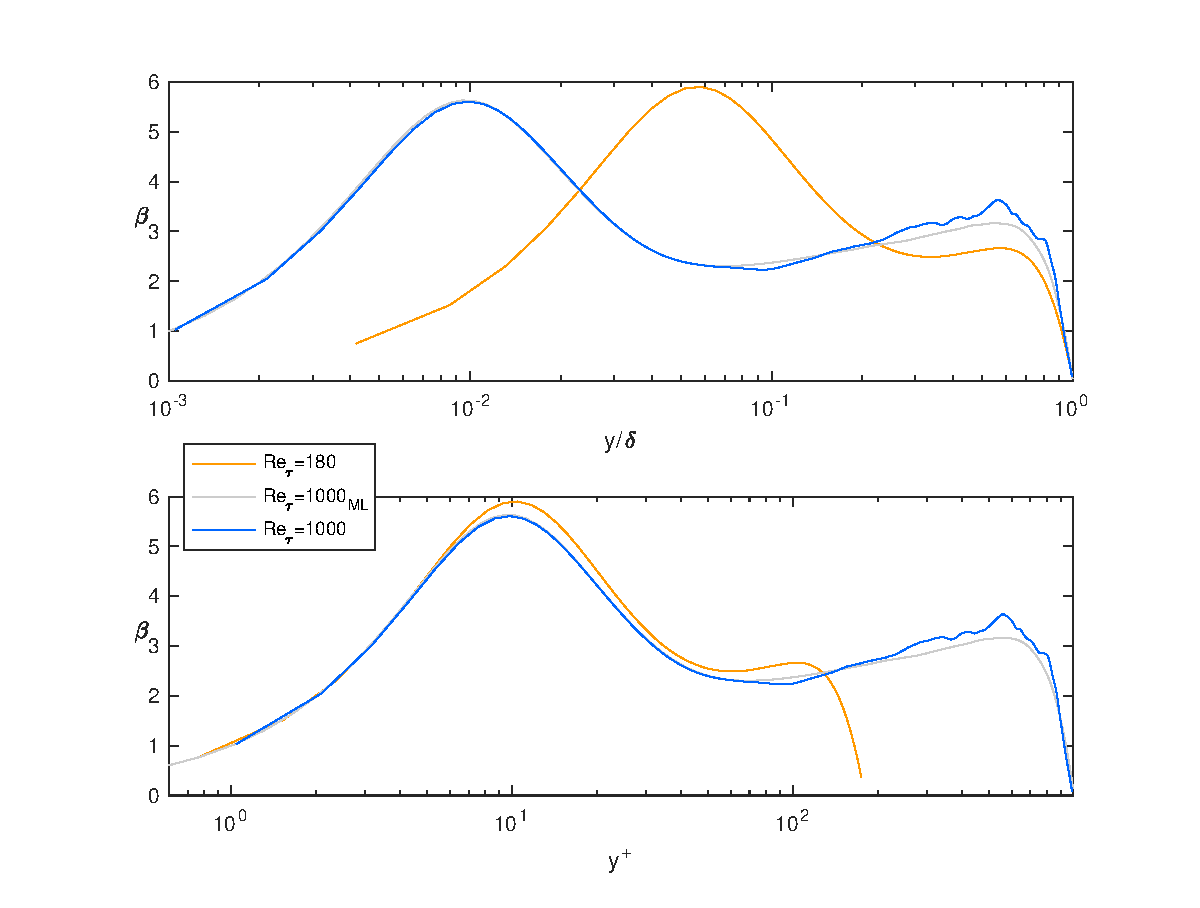
\includegraphics[scale=0.55]{grafici/towsend.eps}
\caption{Logarithmic indicator function applied to mean profile $\langle u \rangle$}
\label{towsend}
\end{center}
\end{figure}

The same indicator function can be applied also to the mean profile for the same purpose, in this case it is a common practice to indicate the function with $\beta$. In figure~\ref{towsend} we reported the comparison against our two simulation and the simulation at $Re_{\tau}=1000$ made by Moser and Lee, in inner and outer scaling. Aside the outer region in which our $Re_{\tau}=1000$ simulation exhibit strong fluctuations, the fitting of the two results is good.

Comparing the behavior of the \emph{rms} in the homogeneous directions, observing~\ref{uu:comparison}\emph{b} and~\ref{ww:comparison}\emph{b}, we can affirm that, while $u'^{2}$ exhibit a little upward shift in its values and a rigid shift towards the wall, $w'^{2}$ grows in all its aspects, with the peak that becomes more prominent and moves closer to the wall. \par
The trailing part of the curve however is still higher than the peak of the $Re_{\tau}=180$ simulation, enclosing it. To sum up we can affirm that the raise in Reynolds number seems to be more effective on the spanwise fluctuating term, instead of the streamwise ones.\\~\par


The graph~\ref{vv:comparison} shows the wall-normal fluctuations, expressed as always in function of $y/\delta$ and $y^{+}$.\par
As we can catch from the plot the blue curve exhibit higher values of fluctuations, distributed across a wider range of length scales than the orange ones. This expected behavior is associated to the higher turbulence content at which the flow is subjected. \par
A remarkable difference against figure~\ref{ww:comparison}\emph{a},~\ref{uu:comparison}\emph{a} and figure~\ref{vv:comparison}\emph{a} is the shift of the $Re_{\tau}=1000$ peak towards higher values of $y^{+}$. \\~\par

A similar peak trend can be recovered also in figure~\ref{uv:comparison}. Such figure report the product of the fluctuations among the streamwise and spanwise directions, which is directly involved in the processes of \emph{production} and stress generation.\par
The curves tend to raise their peak as the Reynold number becomes larger, thus increasing the already cited processes. The net movement of the peak towards the wall, shown in graph~\ref{uv:comparison}\emph{b}, is responsible for the leftward movement of the normalized Reynolds stress of figure~\ref{shear:comparison}.
Once again there are no evidence of logarithmic regions. \\~\par

We summarized few quantities at $Re_{\tau}$ variation in table~\ref{quantities:Re}.\\~\par

\begin{table}[h]
\caption{Significant quantities at $Re_{\tau}$ variation}
\begin{center}
\begin{tabular}{cccccccc}
\toprule
$\mathbf{Re_{\tau}}$ & $\mathbf{Re_{b}}$ & $\mathbf{U_{b}}$ & $\mathbf{U_{c}}$ & $\mathbf{u'^{2}_{peak}}$ & $\mathbf{w'^{2}_{peak}}$ & $\mathbf{v'^{2}_{peak}}$ & $\mathbf{-u'v'_{peak}}$\\
\hline
$\mathbf{180}$ & $5600$ & 15.66 & 18.25 & 7.02 & 1.19 & 0.71 & 0.72 \\
$\mathbf{1000}$ & $40000$ & 19.99 & 22.75 & 8.06 & 2.21 & 1.22 & 0.91 \\
\bottomrule
\end{tabular}
\end{center}
\label{quantities:Re}
\end{table}

\begin{figure}
\begin{center}
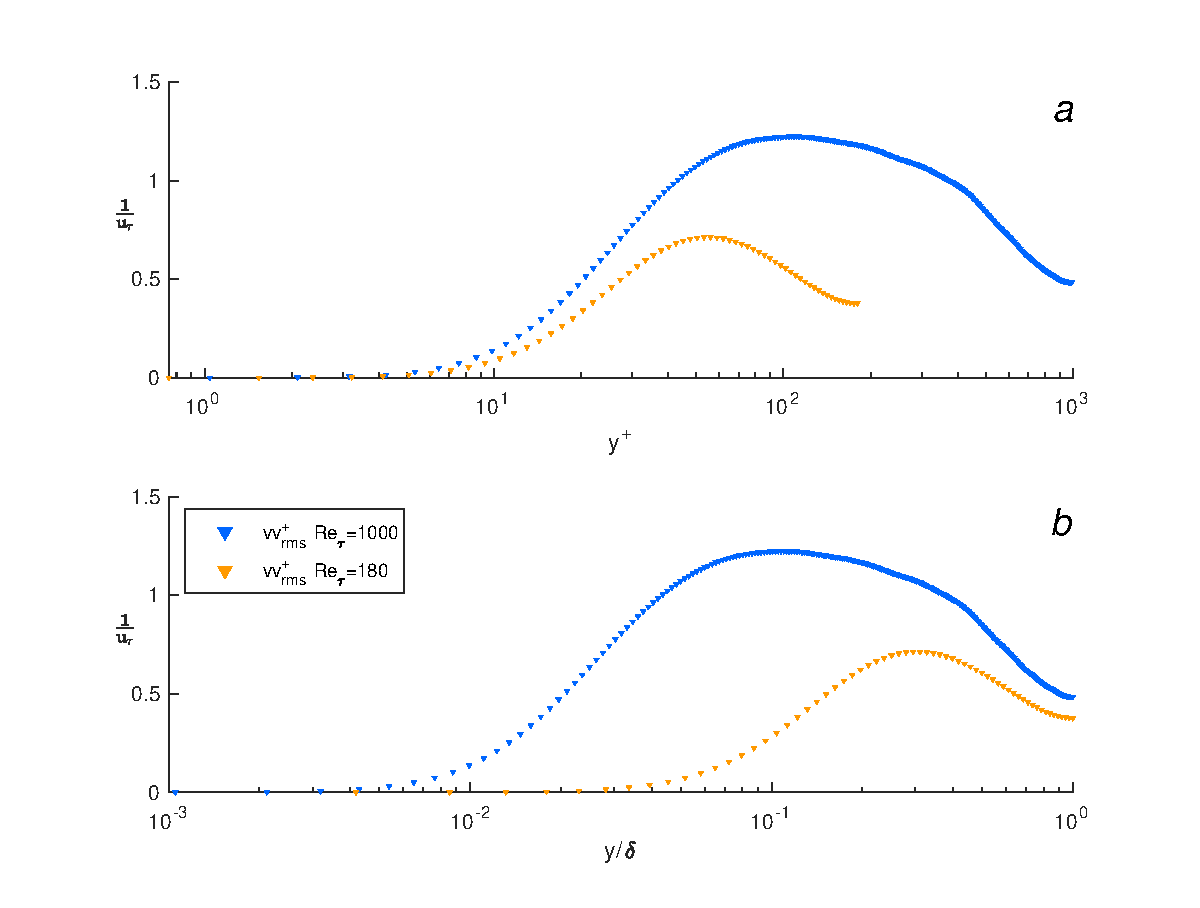
\includegraphics[scale=0.55]{grafici/vv_comparison}
\caption{Wall-normal fluctuations as function of the distance from the wall, plotted at $Re_{\tau}$ variation}
\label{vv:comparison}
\end{center}
\end{figure}

\begin{figure}
\begin{center}
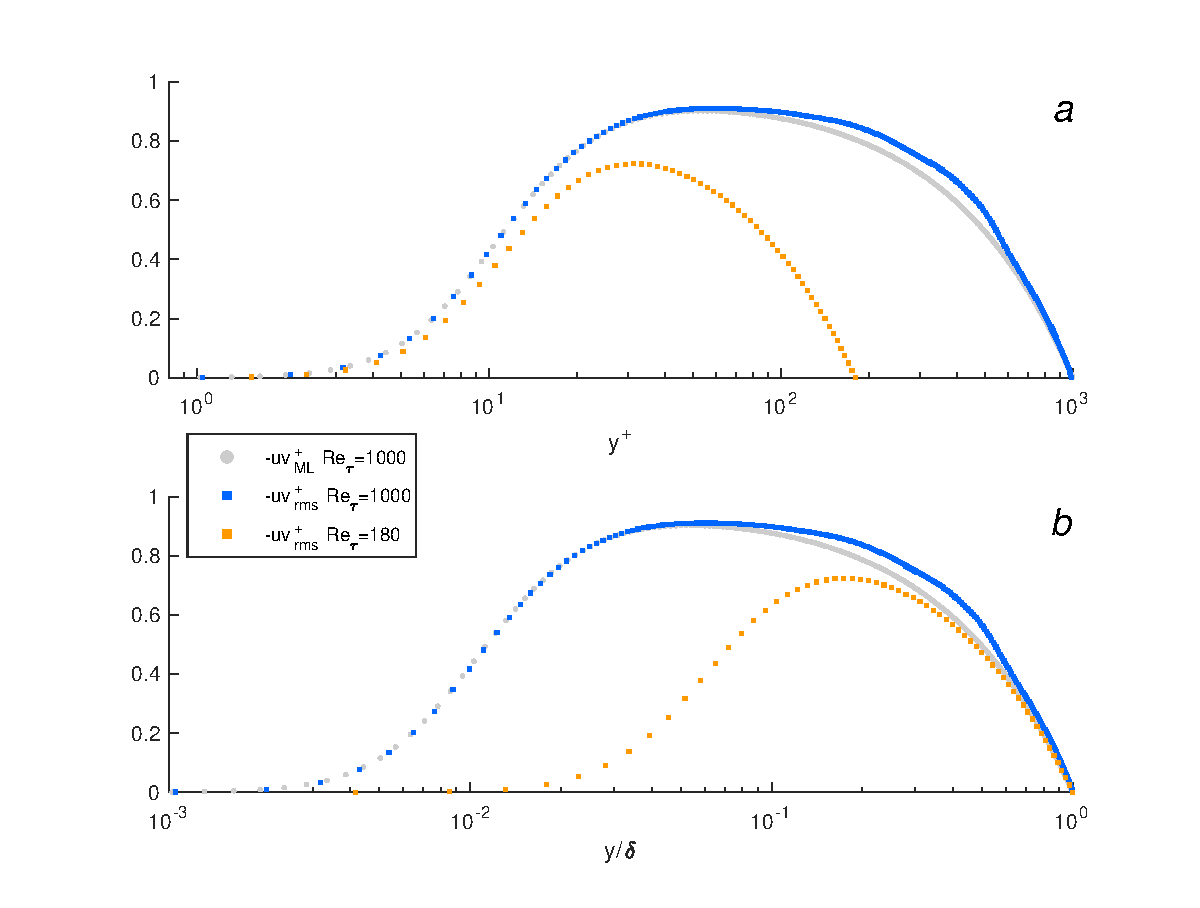
\includegraphics[scale=0.55]{grafici/uv_comparison}
\caption{$-u'v'$ as function of the distance from the wall, plotted at $Re_{\tau}$ variation}
\label{uv:comparison}
\end{center}
\end{figure}

